\section{Sprint 4 – Stats \& Deployment}

In this section, we first present the Sprint 4 backlog, then detail the design and implementation of key features through screenshots and diagrams.

\subsection{Sprint 4 Backlog}
 
\begin{table}[!htbp]
  \centering
  \small
  \caption{Sprint 4 Backlog}
  \label{tab:backlog_sprint4}
  \begin{tabular}{|p{1cm}|p{5cm}|p{6cm}|p{2cm}|}
    \hline
    \textbf{ID} & \textbf{User Story} & \textbf{Description} & \textbf{Priority} \\ \hline
    US10 & View spending analytics & As a corporate user, I want to view comprehensive spending analytics to understand transaction patterns and credit usage across my organization. & Critical \\ \hline
    US11 & Generate financial reports & As a corporate user, I want to generate detailed financial reports for compliance and business analysis purposes. & High \\ \hline
    US12 & CI/CD pipeline optimization & As a development team, we want automated testing, building, and deployment pipelines to ensure rapid and reliable releases. & High \\ \hline
  \end{tabular}
\end{table}

\subsection{Use Case Diagram}

Figure~\ref{fig:uc_sprint4} presents the new use cases for Sprint 4, including spending analytics viewing, financial report generation, and system deployment activities.

\begin{figure}[H]
  \centering
  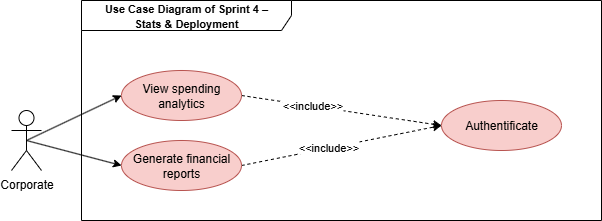
\includegraphics[width=0.75\textwidth]{images/usecase_sprint4.png}
  \caption{Use Case Diagram – Sprint 4}
  \label{fig:uc_sprint4}
\end{figure}

\subsection{Use Case Descriptions – Sprint 4}

In this section, we detail each use case identified for Sprint 4.

\vspace{5cm}

\subsubsection{Use Case "View spending analytics"}
\begin{longtable}{|p{0.2\textwidth}|p{0.75\textwidth}|}
  \caption{Description of use case "View spending analytics"}
  \label{tab:uc_view_analytics} \\
  \hline
  \textbf{Title} & View spending analytics \\ \hline
  \textbf{Actors} & Corporate \\ \hline
  \textbf{Description} & Corporate user views comprehensive spending analytics to understand transaction patterns, credit usage, and organizational financial behavior. \\ \hline
  \textbf{Preconditions} & 
    \begin{itemize}[nosep,leftmargin=*]
      \item Corporate user is authenticated with analytics access permissions.
      \item Historical transaction data is available in the analytics system.
      \item Analytics controller is operational and responsive.
    \end{itemize} \\ \hline
  \textbf{Postconditions} & 
    \begin{itemize}[nosep,leftmargin=*]
      \item Analytics data is retrieved and displayed in interactive charts.
      \item Corporate user can filter and analyze spending patterns.
      \item Analytics viewing activity is logged for audit purposes.
    \end{itemize} \\ \hline
  \textbf{Main Scenario} &
    \begin{enumerate}[nosep,leftmargin=*]
      \item Corporate user requests to display analytics dashboard.
      \item Analytics interface submits request to analytics controller.
      \item Analytics controller processes request and retrieves data.
      \item System returns analytics data to the interface.
      \item Interface displays spending data in charts and graphs.
      \item Corporate user can interact with analytics and apply filters.
    \end{enumerate} \\ \hline
  \textbf{Alternative Scenarios} &
    \begin{enumerate}[nosep,leftmargin=*]
      \item If no analytics data exists, display "No spending data available".
      \item If date range filter returns no results, show "No data for selected period".
    \end{enumerate} \\ \hline
  \textbf{Exception Scenarios} &
    \begin{enumerate}[nosep,leftmargin=*]
      \item If analytics service returns exception, pass error message to interface.
      \item If data processing fails, display "Failed to load analytics data".
      \item If network timeout occurs, show "Connection timeout, please retry".
    \end{enumerate} \\ \hline

\end{longtable}

\vspace{5cm}

\subsubsection{Use Case "Generate financial reports"}
\begin{longtable}{|p{0.2\textwidth}|p{0.75\textwidth}|}
  \caption{Description of use case "Generate financial reports"}
  \label{tab:uc_generate_reports} \\
  \hline
  \textbf{Title} & Generate financial reports \\ \hline
  \textbf{Actors} & Corporate \\ \hline
  \textbf{Description} & Corporate user generates comprehensive financial reports for compliance, auditing, and business analysis purposes with detailed transaction summaries. \\ \hline
  \textbf{Preconditions} & 
    \begin{itemize}[nosep,leftmargin=*]
      \item Corporate user is authenticated with report generation permissions.
      \item Financial data is available in the analytics system.
      \item Report generation service is operational.
    \end{itemize} \\ \hline
  \textbf{Postconditions} & 
    \begin{itemize}[nosep,leftmargin=*]
      \item Financial report is generated and available for download.
      \item Report generation activity is logged for compliance.
      \item Corporate user receives confirmation of successful report creation.
    \end{itemize} \\ \hline
  \textbf{Main Scenario} &
    \begin{enumerate}[nosep,leftmargin=*]
      \item Corporate user requests to generate financial reports.
      \item Analytics interface submits report generation request.
      \item Analytics controller processes request and compiles data.
      \item System returns compiled report data to interface.
      \item Interface displays report data and provides download options.
      \item Corporate user can download or view the generated report.
    \end{enumerate} \\ \hline
  \textbf{Alternative Scenarios} &
    \begin{enumerate}[nosep,leftmargin=*]
      \item If report generation takes time, show progress indicator.
      \item If user cancels generation, stop processing and return to dashboard.
    \end{enumerate} \\ \hline
  \textbf{Exception Scenarios} &
    \begin{enumerate}[nosep,leftmargin=*]
      \item If analytics service returns exception, pass error message to interface.
      \item If report generation fails, display "Report generation failed, please retry".
      \item If insufficient data exists, show "Insufficient data for report generation".
    \end{enumerate} \\ \hline

\end{longtable}

\subsection{Sequence Diagrams}

\subsubsection{Sequence Diagram - View Spending Analytics}
This diagram (see figure \ref{fig:seq_view_analytics}) models the spending analytics viewing process with data retrieval and display:
\begin{itemize}[nosep,leftmargin=*]
  \item Corporate user requests to display analytics data.
  \item Analytics interface submits request to analytics controller.
  \item Controller processes request and retrieves analytics data.
  \item System returns data for display in interactive charts.
  \item Error handling provides appropriate feedback for failures.
\end{itemize}

\begin{figure}[H] 
  \centering
  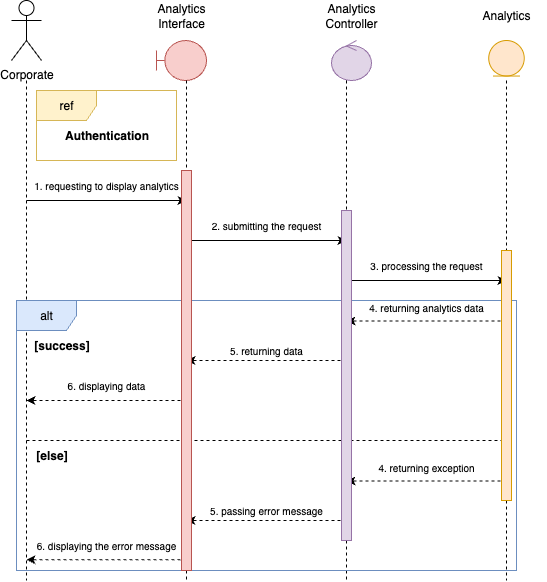
\includegraphics[width=\textwidth,keepaspectratio]{images/seq_view_spending_analytics.png}
  \caption{Sequence Diagram "View Spending Analytics"}
  \label{fig:seq_view_analytics}
\end{figure}

\subsubsection{Sequence Diagram - Generate Financial Reports}
This diagram (see figure \ref{fig:seq_generate_reports}) shows the financial report generation process with data compilation:
\begin{itemize}[nosep,leftmargin=*]
  \item Corporate user requests financial report generation.
  \item Analytics interface forwards request to analytics controller.
  \item Controller processes and compiles financial data into reports.
  \item System returns compiled report data for download or viewing.
\end{itemize}

\begin{figure}[H] 
  \centering
  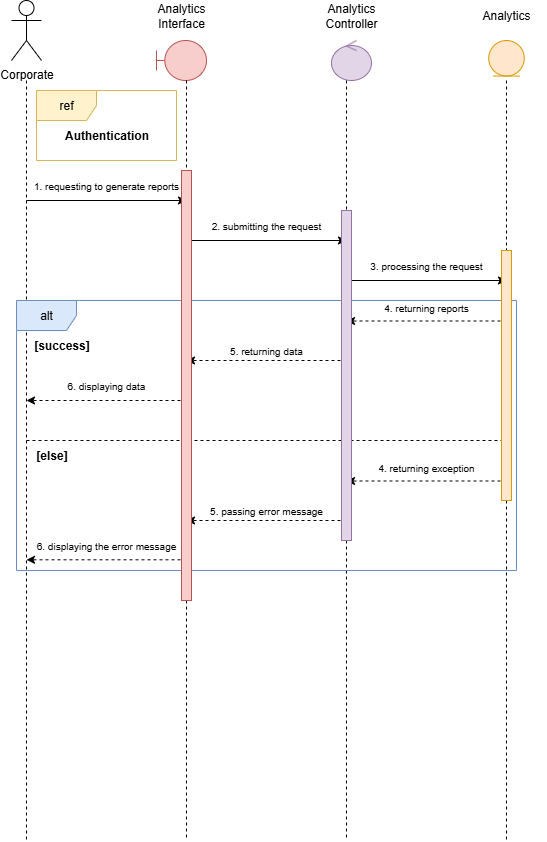
\includegraphics[width=\textwidth,keepaspectratio]{images/seq_generate_financial_reports.png}
  \caption{Sequence Diagram "Generate Financial Reports"}
  \label{fig:seq_generate_reports}
\end{figure}

\subsection{Class Diagram (Sprint 4)}

The enriched class diagram for Sprint 4 adds new entities for analytics and reporting:

\begin{itemize}[nosep,leftmargin=*,label=—]
  \item \textbf{SpendingAnalytics}: manages spending analytics data and calculations.
    \begin{itemize}[nosep,leftmargin=*]
      \item \texttt{id}: unique identifier for analytics record;
      \item \texttt{corporateId}: associated corporate account identifier;
      \item \texttt{period}: time period for analytics (DAILY, WEEKLY, MONTHLY);
      \item \texttt{totalSpending}: total spending amount for the period;
      \item \texttt{transactionCount}: number of transactions in period;
      \item \texttt{averageTransaction}: average transaction amount;
      \item \texttt{generatedAt}: timestamp of analytics generation.
    \end{itemize}

  \item \textbf{FinancialReport}: comprehensive financial reporting for compliance and analysis.
    \begin{itemize}[nosep,leftmargin=*]
      \item \texttt{id}: unique report identifier;
      \item \texttt{corporateId}: corporate account for the report;
      \item \texttt{reportType}: type of report (SPENDING, COMPLIANCE, AUDIT);
      \item \texttt{startDate}: report period start date;
      \item \texttt{endDate}: report period end date;
      \item \texttt{generatedAt}: report generation timestamp;
      \item \texttt{filePath}: path to generated report file;
      \item \texttt{status}: report generation status.
    \end{itemize}
\end{itemize}

% \begin{figure}[htbp]
%   \centering
%   \includegraphics[width=1\textwidth]{images/class_diagram_sprint4.png}
%   \caption{Class Diagram – Sprint 4}
%   \label{fig:class_sprint4}
% \end{figure}

\vspace{20cm}

\subsection{CI/CD Pipeline Implementation}

To ensure rapid and reliable delivery of Credix enhancements, we implemented comprehensive CI/CD pipelines for both frontend and backend components using GitHub Actions and Docker.

\noindent\textbf{*GitHub Actions Pipeline:}

The workflow file \texttt{.github/workflows/ci-cd.yml} (see figure \ref{fig:github_actions_workflow}) defines the pipeline stages: code checkout, dependency installation, testing, building, and deployment to production.

% \begin{figure}[H]
%   \centering
%   \includegraphics[width=\textwidth,keepaspectratio]{images/github_actions_workflow.png}
%   \caption{GitHub Actions CI/CD workflow configuration}
%   \label{fig:github_actions_workflow}
% \end{figure}
% \FloatBarrier

\noindent\textbf{*GitHub Repository:}

The GitHub repository (see figure \ref{fig:github_repo_credix}) shows the automated workflow triggers on main branch commits, with status badges indicating build health.

% \begin{figure}[H]
%   \centering
%   \includegraphics[width=\textwidth,keepaspectratio]{images/github_repo_credix.png}
%   \caption{GitHub repository with CI/CD workflow status}
%   \label{fig:github_repo_credix}
% \end{figure}
% \FloatBarrier

\noindent\textbf{*Docker Containerization:}

The \texttt{Dockerfile} (see figure \ref{fig:dockerfile_credix}) enables consistent deployment across environments with optimized multi-stage builds.

% \begin{figure}[H]
%   \centering
%   \includegraphics[width=0.7\textwidth,keepaspectratio]{images/dockerfile_credix.png}
%   \caption{Dockerfile for Credix application containerization}
%   \label{fig:dockerfile_credix}
% \end{figure}
% \FloatBarrier

\noindent\textbf{*Production Deployment:}

The production environment (see figure \ref{fig:production_deployment}) runs on cloud infrastructure with automated scaling and monitoring.

% \begin{figure}[H]
%   \centering
%   \includegraphics[width=\textwidth,keepaspectratio]{images/production_deployment_credix.png}
%   \caption{Production deployment dashboard showing system health}
%   \label{fig:production_deployment}
% \end{figure}
% \FloatBarrier

\subsection{Realization (Sprint 4)}

This section presents the interfaces and features implemented during Sprint 4, focusing on spending analytics, financial reporting, and deployment capabilities. Each interface is illustrated with screenshots and accompanied by functionality descriptions.

\subsubsection{Spending analytics dashboard}

The spending analytics dashboard provides comprehensive visualization of organizational spending patterns and credit usage (see Figure \ref{fig:analytics_dashboard}).

% \begin{figure}[H]
%   \centering
%   \includegraphics[width=\textwidth,keepaspectratio]{images/spending_analytics_dashboard.png}
%   \caption{Spending Analytics Dashboard}
%   \label{fig:analytics_dashboard}
% \end{figure}

— \textbf{States presented:}
\begin{itemize}[nosep,leftmargin=*,label=•]
  \item \textbf{Interactive charts}  
    Visual representation of spending patterns with drill-down capabilities.
  \item \textbf{Time period filters}  
    Selection of daily, weekly, monthly, or custom date ranges.
  \item \textbf{Category breakdown}  
    Spending analysis by transaction type and user groups.
  \item \textbf{Trend analysis}  
    Historical trends and predictive spending insights.
\end{itemize}

— \textbf{Analytics viewing flow:}
\begin{itemize}[nosep,leftmargin=*,label=•]
  \item Corporate user accesses analytics dashboard.
  \item System retrieves and processes historical transaction data.
  \item Analytics controller compiles spending metrics and patterns.
  \item Interface displays interactive charts and filtering options.
  \item User can explore data through various visualization options.
\end{itemize}

\subsubsection{Financial reporting interface}

The financial reporting interface enables generation of comprehensive reports for compliance and business analysis (see Figure \ref{fig:financial_reports}).

% \begin{figure}[H]
%   \centering
%   \includegraphics[width=\textwidth,keepaspectratio]{images/financial_reporting_interface.png}
%   \caption{Financial Reporting Interface}
%   \label{fig:financial_reports}
% \end{figure}

— \textbf{States presented:}
\begin{itemize}[nosep,leftmargin=*,label=•]
  \item \textbf{Report type selection}  
    Choice of spending reports, compliance reports, or audit trails.
  \item \textbf{Date range configuration}  
    Flexible date range selection for report generation.
  \item \textbf{Export options}  
    Multiple format options (PDF, Excel, CSV) for report download.
  \item \textbf{Report history}  
    Access to previously generated reports and templates.
\end{itemize}

— \textbf{Report generation flow:}
\begin{itemize}[nosep,leftmargin=*,label=•]
  \item Corporate user selects report type and parameters.
  \item System compiles financial data based on specified criteria.
  \item Analytics controller processes and formats report data.
  \item Generated report is made available for download or viewing.
  \item Report generation activity is logged for compliance tracking.
\end{itemize}
